%% This is a JAIR Example File Compiled by Nicholas Mattei (nsmattei@tulane.edu) 
%% and Odd Erik Gundersen (odderik@ntnu.no)
%% and Mykel Kochenderfer (mykel@stanford.edu)
%% September 15, 2025
%%
%% This file is based off the ACM Latex Template https://www.acm.org/publications/proceedings-template
%% Revision 2.12 (12/28/2024)
%% 
%% Please see https://www.jair.org/index.php/jair for more information and submission instructions.
%%

%% The first command in your LaTeX source must be the \documentclass
%% command.
%%
%% For submission and review of your manuscript please change the
%% command to \documentclass[manuscript, screen, review]{jair}.
%%
\documentclass[]{jair}

\usepackage[T1]{fontenc}
\usepackage{url}
\usepackage{algorithm,algpseudocode}
\usepackage{amsthm}
\newtheorem{Theorem}{Theorem}
\newtheorem{Definition}{Definition}

\makeatletter
\AtBeginDocument{%
  \fancyfoot[RO,LE]{}%
  \fancypagestyle{firstpagestyle}{%
    \fancyhf{}%
    \fancyfoot[RO,LE]{}%
  }%
}
\makeatother

\setcopyright{cc}
\copyrightyear{2025}
\acmDOI{10.1613/jair.1.xxxxx}

%%
\JAIRAE{Insert JAIR AE Name}
\JAIRTrack{} % Insert JAIR Track Name only if part of a special track

\RequirePackage[
  datamodel=acmdatamodel,
  style=acmauthoryear,
  backend=biber,
  giveninits=true,
  uniquename=init
  ]{biblatex}

\renewcommand*{\bibopenbracket}{(}
\renewcommand*{\bibclosebracket}{)}

%%
%% For managing citations, use BibLaTeX with the acmauthoryear style.
%% The next line specifies the bibliography file.
\addbibresource{references.bib}

%%
%% end of the preamble, start of the body of the document source.
\begin{document}

%%
%% The "title" command has an optional parameter,
%% allowing the author to define a "short title" to be used in page headers.
%\title{JAIR Example Template}
\title[LTLplanning]{Locality-based moral planning with linear temporal logic values}

%%
%% The "author" command and its associated commands are used to define
%% the authors and their affiliations.
%% Of note is the shared affiliation of the first two authors, and the
%% "authornote" and "authornotemark" commands
%% used to denote shared contribution to the research and/or corresponding author.


\author{Adrian Satja Kurdija}
\authornote{Corresponding Author.}
\orcid{0000-0003-2313-0396}
\email{adrian.kurdija@fer.unizg.hr}
\affiliation{%
  \institution{Faculty of Electrical Engineering and Computing, University of Zagreb}
  \city{Zagreb}
  \country{Croatia}
}

\author{Matej Mihel\v{c}i\'{c}}
\orcid{0000-0002-1023-8413}
\email{matmih@math.hr}
\affiliation{%
  \institution{Department of Mathematics, Faculty of Science, University of Zagreb }
  \city{Zagreb}
  \country{Croatia} 
  }
  \email{matej.mihelcic@irb.hr}
\affiliation{%
  \institution{Department of Electronics, Ru\dj er Bošković Institute }
  \city{Zagreb}
  \country{Croatia} 
  }

%% The short list of authors must be made of the list of all authors' lastnames.
\renewcommand{\shortauthors}{Kurdija and Mihelčić}
%% If this is too long and overlaps other information printed in the page headers, use
%\renewcommand{\shortauthors}{Xu et al.}

%%
%% The abstract is a short summary of the work to be presented in the
%% article.
\begin{abstract}
\textbf{Objective:} We study the CONFLICT problem in logic-based ethical planning with Linear Temporal Logic (LTL) values, which is PSPACE-complete in general, and target a tractable fragment relevant to structured robotic domains.

\textbf{Method:} We introduce locality assumptions over propositions and actions: most propositions are indexed along an ordered local axis, each action depends on and modifies only a bounded interval, the number of global propositions is constant, and locality also constrains feasible temporal action order. Under these assumptions, we derive a polynomial-time locality-based planning algorithm.

\textbf{Results:} We evaluate against brute-force and automata/progression baselines on a deterministic 110-instance benchmark suite spanning three modeled robotic families (linear traffic lights, charging extension, and narrow three-lane corridor). With a common 15-second timeout and independent validation, the locality planner solves 110/110 instances, while automata/progression solves 105/110 and brute force 90/110. The locality method also has the lowest runtime distribution and significantly smaller per-instance runtimes in one-sided Mann--Whitney U tests.

\textbf{Conclusion:} Locality-aware state compression yields a practically robust and fast exact planner in high-locality domains, while retaining expressive temporal value constraints.
\end{abstract}

%\begin{abstract}
%      A clear and well-documented \LaTeX\ document is presented as an
%  article formatted for publication by ACM in a conference proceedings
%  or journal publication. Based on the ``acmart'' document class, this
%  article presents and explains many of the common variations, as well
%  as many of the formatting elements an author may use in the
%  preparation of the documentation of their work.
%\end{abstract}


%% JAIR Note: 
%% Do not include ACM CCS Concepts or Keywords


%% To be updated by authors.
\received{}
\received[accepted]{}

%%
%% This command processes the author and affiliation and title
%% information and builds the first part of the formatted document.
\maketitle

\section{Introduction}

Planning is crucial for autonomous systems like robotics. A framework for logic-based ethical planning with intended application to robotics was introduced by Grandi et al. \cite{grandi2022logic}. For a key problem, which is to ensure that actions of an agent align with multiple predefined (moral or other) values, linear temporal logic is used to represent values and determine feasible action plans. Evaluation criteria for individual plans were proposed in \cite{grandi2023moral}. General propositional planning problems (ie, PLANSAT) are known to be PSPACE-complete \cite{BYLANDER1994165}, as well as the problem of moral conflict as defined in Grandi et al. \cite{grandi2022logic}. In this work we introduce locality-based constraints of actions and propositions to reduce the search space and computational complexity. 

Linear Temporal Logic (LTL) enables specifying constraints over sequences of actions \cite{10.5555/975331}.
A set of moral values $\Omega$ consists of LTL formulas \cite{4567924} that describe temporal properties of atomic propositions (evaluated under some history $H$) using operators such as negation ($\neg \phi$), conjunction ($\phi_1\land \phi_2$), "next" ($X\phi$), "until" ($\phi_1 \sf{U} \phi_2$), "henceforth" ($G\phi$), and "eventually" ($F\phi$). For a given moral problem consisting of moral values $\Omega$, action theory $\gamma$, and an initial state $s_0$, the CONFLICT problem asks if there is an action plan $\pi$ satisfying all values from $\Omega$. If there is no such action plan, some values have to be broken, so tradeoffs between values have to be accounted for, which explains the name {\it moral conflict}. However, we note that the concerned values do not have to be ethical/moral in the strict sense of the word. We decided to follow the previous terminology while keeping in mind the generality of the approach.


Grandi et al. \cite{grandi2022logic} have shown that several planning tasks are intractable (PSPACE-complete). Namely, CONFLICT is shown to be PSPACE-complete using reduction from the propositional STRIPS planning problem called PLANSAT \cite{BYLANDER1994165}. The difficulty of the problem arises from the exponential number of possible plans.
Using additional assumptions at the cost of generality, we define a constrained version of the CONFLICT problem and present the algorithm to solve it. Namely, to enable polynomial complexity, we restrict actions to affect only a local set of propositions, introducing the {\it locality} assumption. 

The proposed framework allows modelling many real-world scenarios involving planning. One example includes utilizing propositions to express properties involving linear space order. Many robots involved in repairs or manufacturing adhere to such constraints (e.g. robots used to pick and pack food in the factories, gantry robots used in automotive industry, robots dispatching pallets in the warehouses, robots in electronic chip manufacturing or pharmaceutical production). Utilizing proposed logic, these robots could move back and forth satisfying expressive, complex constraints. One important constraint is not to harm human workers that might cross the path of the traversing robots. This shows the importance of having the possibility to add moral constraints in the planning process  to create safe, flexible and efficient robots.    
To complement the theoretical analysis, we perform an empirical comparison against brute-force and automata/progression baselines on systematic instances derived from the three examples in this paper, reporting both runtime and completion behavior under equal timeout budgets.

The paper is organized as follows. Sect. \ref{related} describes the related work. In Sect. \ref{lbp} we describe the framework and the proposed algorithm. In Sect. \ref{example} we present examples. Sect. \ref{eval} reports benchmark-based evaluation. Conclusions are given in Sect. \ref{conc}.
\section{Related Work}\label{related}

Logic-based temporal planning has previously been studied in the context of robotics and autonomous systems. Various approaches have been used to address uncertainty, efficiency, and fairness in decision-making. Significant focus has been on using LTL, as well as probabilistic temporal logic \cite{konur2011realtimeprobabilistictemporallogics}, to define and schedule complex tasks in dynamic and uncertain environments. 
Earlier work such as \cite{fainekos2009temporal} investigated temporal logic motion planning for dynamic robots, formulating a hierarchical approach that integrates motion tracking and formal logic specifications to satisfy high-level tasks. Research \cite{cai2024reinforcement} explored methods based on reinforcement learning (RL) to satisfy soft temporal logic constraints in environments where full compliance is not feasible due to motion uncertainties and environmental uncertainties.
Some works have investigated probabilistic and reactive planning frameworks. Yoo et al. \cite{yoo2013probabilistic} introduced a probabilistic computation tree logic (PCTL) extension to incorporate resource constraints in motion planning, while Cai et al. \cite{cai2021probabilistic} developed a probabilistic LTL motion planning strategy that takes into account both environmental uncertainties and motion uncertainties. In contrast, Zhou et al. \cite{kan2024local} proposed local observation-based reactive temporal logic planning, focusing on real-time human-robot interactions.

While heuristic search and approximate methods—such as those utilizing reinforcement learning to satisfy soft temporal logic constraints or probabilistic LTL frameworks—offer scalability in uncertain or highly unconstrained environments, they often inherently sacrifice strict guarantees of value satisfaction. In safety-critical robotic applications, such as robots performing tasks in the presence of human workers, approximate compliance is simply insufficient because a potential collision could cause serious injury or fatality. Our approach contrasts directly with these heuristic methods by providing an exact planning algorithm. By exploiting the inherent structural locality of specific operational domains, we achieve the computational efficiency typically associated with approximate methods—specifically, polynomial-time solvability—without relinquishing the absolute mathematical guarantees required for strict moral and safety compliance.

A related research area has been automated reasoning and decision-making for autonomous systems. Meli et al. \cite{melilogic} have employed logic programming to improve deliberative robotic task planning, allowing robots to efficiently evaluate and execute high-level actions.
Meanwhile, Shea-Blymyer and Abbas \cite{10.1145/3460975} have formalized {\it algorithmic ethics} for autonomous systems, introducing a framework based on deontic logic \cite{von1951deontic} to satisfy regulatory and ethical constraints. Similarly, 
 Liang and Vasile \cite{fairplanning} addressed concerns about fairness in Mobility-on-Demand systems by using fairness metrics based on temporal logic in decision-making algorithms.
In recent work, the use of automata-based approaches has appeared, such as Toscano-Moreno et al. \cite{li2024spin} which proposed SPIN-based LTL path planning, utilizing model checking for efficient motion planning in environments with uneven terrain. Huang et al. \cite{HUANG2026131593} proposed the \emph{DriveLegal}, a modular legal-interpretation framework for downstream autonomous driving applications, based on Large Language Models (LLMs) to improve legal interpretation for autonomous vehicle decision making.

A particularly relevant line of work for finite-trace temporal planning is automata/product-state search for $LTL_f$ formulas \cite{degiacomo2013ltlf,camacho2018finite}. Intuitively, the planner keeps two pieces of information at each step: the current world state, and a compact summary of ``what still needs to happen'' for the temporal goals to be satisfied. After every action, this temporal summary is updated; this update is often called progression. Search is then performed over pairs of the form (world state, temporal summary), so two identical world states are treated differently if they have different remaining temporal obligations. The method is general and theoretically clean, but the number of such pairs can grow quickly. Our automata/progression baseline in Section \ref{eval} follows this paradigm, while our main method additionally exploits interval locality to keep the explored state space smaller.

Recent research on $LTL_f$ synthesis aims to find new ways to perform synthesis, such as using satisfiability solvers \cite{favorito2023DPLL, ciao2024synthesis}, where the synthesis problem is encoded into SAT-style reasoning, and solving the problem on the fly \cite{xiao2025fly}, where only the needed fragment of the search space is generated during synthesis. Interesting research directions include solving reactive problems with nondeterministic domains \cite{duret2025engineering}, where the environment may respond in multiple possible ways to the same action, solving adaptive synthesis problems, where the agent tries to satisfy as many goals as possible at any moment of execution \cite{giacomo2025}, and synthesis under unreliable inputs \cite{hagemeier2025}, where it is assumed that agent's sensory data cannot be fully trusted and thus backup plans are devised. De Giacomo et al. \cite{giacomoResp2025} introduced the notion of responsibility anticipation and attribution in $LTL_f$ synthesis, where agents' actions are evaluated both before and after an action is performed. We believe that our locality-based theory can be incorporated and highly beneficial in many of these settings since many problems involving agents naturally adhere to the incorporated constraints and due to exceptional speed in which existence of satisfying plans can be detected. %add if we create a polynomial algorithm for max plan or similar  

\section{Locality-Based Planning}\label{lbp}

Section \ref{lbep} describes the relevant part of the framework defined in \cite{grandi2022logic}, Section \ref{aa} describes our additional assumptions and Section \ref{pa} describes the proposed algorithm.

\subsection{Logic-Based Ethical Planning}\label{lbep}

The world is described by atomic propositions $Prop=\{p_1, \dots, p_n\}$.
Their Boolean truth values are represented as a state $s\in 2^{Prop}$ which
consists of all propositions that are true at a given moment.

Linear Temporal Logic over Finite Traces, noted as \( LTL_{f} \), is a temporal logic used to represent an agent's values and goals over finite traces. \( LTL_{f} \) includes the operators from classical linear temporal logic such as "next" (\( X \)) and "until" (\( U \)), allowing for expressions about the progression of time and the satisfaction of certain conditions. Additionally, the standard operators "henceforth" (\( G \)) and "eventually" (\( F \)) are defined as \( G\varphi := \neg(\top U \neg \varphi) \) and \( F\varphi := \top U \varphi \). Formally, the grammar of \( LTL_{f} \) is defined as follows ($p\in Prop$):
\begin{equation}
    \varphi ::= p \mid \neg \varphi \mid \varphi_1 \land \varphi_2 \mid X \varphi \mid \varphi_1 U \varphi_2 \mid G \varphi \mid F \varphi.
\end{equation}

In this paper, we expand the language with additional logical operators in $LTL_f$, defined as follows:
\begin{equation}
\varphi \lor \psi \equiv \neg(\neg \varphi \land \neg \psi), \quad
\varphi \to \psi \equiv \neg \varphi \lor \psi.
\end{equation}

There is a set $Act$ of {\it actions} and each action $a\in Act$ can change values of some propositions
according to the corresponding preconditions. Formally, we define {\it action theory} as a pair of functions
\begin{equation}\gamma^+, \gamma^- : Act \times Prop \to \mathcal{L}_{PL},\end{equation}
where $\mathcal{L}_{PL}$ is the propositional logic fragment of $LTL_f$.
These functions represent preconditions for the actions. Namely,
after action $a$, proposition $p$ becomes true if the precondition $\gamma^+(a, p)$ is true,
and false if the precondition $\gamma^-(a, p)$ is true. These rules will be formalized in Eq. \eqref{h}.
%However, if neither or both preconditions are true, the truth value of $p$ will not change after action $a$.

A sequence of actions $\pi = (a_1, \dots, a_k)$ is called {\it action plan}.

The described rules of action theory allow us to define a {\it history} $H(\pi, s_0, \gamma)$
generated by an action plan $\pi$ from an initial state $s_0$
under action theory $\gamma$. Namely, $H(\pi, s_0, \gamma)$
is a sequence of states $H_0$, $H_1$, $H_2$, $\dots$, $H_k\in 2^{Prop}$ with $H_0=s_0$. To define how $H_t$ transforms
into $H_{t+1}$, we first define the $\models$ relation: we say that $H, t \models \varphi$ if the formula \( \varphi\in LTL_f \) holds at time point $t$ in the history \( H \). More specifically,
\begin{itemize}
    \item \( H, t \models p \iff p \in H_{t} \)  for atomic propositions $p\in Prop$.
    \item \( H, t \models \neg \varphi \iff H, t \not\models \varphi \).
    \item \( H, t \models \varphi_1 \land \varphi_2 \iff H, t \models \varphi_1 \) and \( H, t \models \varphi_2 \).
    \item \( H, t \models X \varphi \iff H, t+1 \models \varphi \) (ie, \( \varphi \) holds in the next state).
    \item \( H, t \models \varphi_1 U \varphi_2 \iff \) there exists a time \( t' \geq t \) such that \( H, t' \models \varphi_2 \) and for all \( t'' \) with \( t \leq t'' < t' \) it holds that \( H, t'' \models \varphi_1 \) (ie, \( \varphi_1 \) holds until \( \varphi_2 \) becomes true).
    \item \( H, t \models F \varphi \iff \) there exists a time \( t' \geq t \) such that \( H, t' \models \varphi \) (ie, \( \varphi \) holds at some future point, {\it eventually}).
    \item \( H, t \models G \varphi \iff \) for all \( t' \geq t \) it holds that \( H, t' \models \varphi \) (ie, \( \varphi \) holds at every point in the future, {\it henceforth}). %In particular, $H,0\models G\varphi$ means that $\varphi$ {\it always} holds.
\end{itemize}

Now, for each action \( a_t \in \pi \) and corresponding time \( t \), the next state \( H_{t+1} \) is determined according to the action theory \( \gamma \) by updating the propositions in \( H_t \) based on the effects of the action \( a_t \):
\begin{equation}\label{h}
\begin{aligned}
H_{t+1} = \bigg( H_{t} \setminus \{ p \in \mathit{Prop} : H_{t} \models \gamma^-(a_t, p) \} \bigg) \cup \{ p \in \mathit{Prop} : H_{t} \models \gamma^+(a_t, p) \}.
\end{aligned}
\end{equation}

Here, for each proposition $p$, we keep or change its truth value based on \( \gamma^+(a_t, p) \) and \( \gamma^-(a_t, p) \), the positive and negative effect preconditions associated with action \( a_t \).

A set of moral values is given by $\Omega\subseteq LTL_f$.
We say that a given moral problem, defined as a triple $\mathcal{M}=(\Omega, \gamma, s_0)$, 
is a moral conflict if there is no satisfactory action plan. Formally, $\mathcal{M}\in CONFLICT$
if there is no action plan $\pi$ such that the history $H(\pi, s_0, \gamma)$ satisfies all values
from $\Omega$. Formally, an action plan $\pi$ is satisfactory if
\begin{equation}
\forall \varphi \in \Omega, \, \ H(\pi, s_0, \gamma), 0 \models \varphi.
\end{equation}
For example,
\begin{itemize}
    \item $H, 0\models p$ when $p\in s_0$,
    \item $H, 0\models Fp$ when $p$ is {\it eventually} satisfied,
    \item $H, 0\models Gp$ when $p$ is {\it always} satisfied,
    \item $H, 0\models FGp$ when $p$ is {\it ultimately} satisfied, ie, it holds in the last state.
\end{itemize}
If there is no such action plan, some values have to be broken, so tradeoffs between values have to be accounted for, which explains the name {\it moral conflict}.

 Grandi et al. \cite{grandi2022logic} showed that CONFLICT is PSPACE-complete using reduction from the propositional STRIPS planning problem called PLANSAT \cite{BYLANDER1994165}. This means that in the general case,
 the space of all action plans cannot be efficiently searched in order to find a plan satisfying $\Omega$.

\subsection{Locality-Based Moral Conflict}\label{aa}

Our contribution lies in restricting CONFLICT to a polynomially solvable variant using additional assumptions that reduce its generality without sacrificing too much of its practical use. Motivated from various real-world examples concerning planning in what is essentially a 1D or 2D space (roads, warehouses), such as the examples in Sect. \ref{example}, we assume that most propositions -- all except for a constant number of them -- are localized. Formally, we introduce locality as the mapping 
\begin{equation}
    loc: Prop \to \{0,1, \dots, n\},\  
\end{equation}
where locations $1, \dots, n$ represent positions of the {\it local} propositions ($loc(p)>0$),
while the propositions with $loc(p)=0$ are considered {\it global}.
To limit the search space, we posit that there are at most $M$ global propositions and at most $M$
propositions at each position:
\begin{equation}
    \forall i\in\{0,1,\dots,n\},\quad |p\in Prop \; : \; loc(p)=i|\le M.
\end{equation}

Each action $a$ depends on, and changes, only the propositions from an interval of at most $L$ locations,
along with any global propositions. This local interval depends on the action. 
To formalize this constraint, we first define $\mathcal{L}_{PL}^{i, j}$ as a fragment of $\mathcal{L}_{PL}$
containing only propositions $p\in Prop$ such that $loc(p)=0$ or $i\le loc(p)\le j$.
Now, for each action $a\in Act$, we assume that there are natural constants $l(a)$ and $r(a)$, representing the left and right action boundaries, such that: 
\begin{equation}
\begin{aligned}1\le l(a) \le r(a) \le n, \\ r(a)-l(a)< L,\\
\gamma^+(a, p_i),\,\gamma^-(a, p_i)\in \mathcal{L}_{PL}^{l(a), r(a)}, \quad & \forall i\in[l(a),r(a)],\\
\gamma^+(a, p_i)=\gamma^-(a, p_i)=\bot, \quad & \forall i\in [1,n]\setminus[l(a),r(a)].\end{aligned}\end{equation}
Therefore, only the propositions from $\mathcal{L}_{PL}^{l(a), r(a)}$ can be changed by or participate in the preconditions for action $a$.

Additionally, we assume that the local ordering of propositions constrains the temporal order of actions.
Informally, the temporal order of actions is roughly left-to-right with allowed deviations.
If the actions' intervals are sufficiently apart, the action on the first interval must be performed before the action on the second. Formally, if $r(b)-l(a)\ge 2L$, then action $a$ cannot be performed after action $b$.
A larger value of $L$ permits more flexibility in the order of actions.
In terms of the action plan $\pi = (a_1, \dots, a_k)$ this condition can be written as
\begin{equation}r(a_j)-l(a_i)\ge 2L \implies i<j.\label{k}\end{equation}

The final constraint is that the value set $\Omega$ contains only formulas with at most one of the operators
$F$, $G$, $FG$, or $U$, operating on a propositional logic formula containing at most $K$ atomic propositions, % (or their negations),
either all local, or all global. In the local case, the absolute difference between their indices can be at most $L$.

The integers $K$, $L$, $M$ are introduced as fixed constants to limit the search space,
and therefore the algorithm complexity. As a reminder,
$K$ is the maximum number of propositions in each value formula,
$L$ is the maximum number of local propositions each action can influence,
and $M$ is the maximum number of global propositions and propositions at each location.
For simplicity of complexity analysis, we will assume that $K, L= O(M)$.

\subsection{Proposed Algorithm}\label{pa}

Under the above assumptions, CONFLICT can be solved in polynomial time. 
The basic idea stems from the temporal constraint:
    $$r(b)-l(a)\ge 2L \implies a \text{ precedes } b,$$ which means
that if action \( a \) uses/changes \( p_i \),
this action precedes all actions \( b \) such that \( r(b) \geq i + 2L \).
Thus, while performing an action plan, we do not need to keep track of "distant" propositions.
We only need to keep track of the truth values of the current $2L$-length interval of
local propositions (called {\it mutable})
and move it left-to-right, along with the global propositions.
The algorithm searches for a path over these substates and the number of such substates is linear in $n$. 

To be able to check the validity of formulas with several local propositions, we must additionally keep track of {\it recent} local propositions (for which $loc(p)\in\langle i-L,i]$) to the left of the currently {\it mutable} interval $[i+1, i+2L]$. The truth value of the recent propositions can no longer be changed, but can play a role in validating (or invalidating) formulas where at least one proposition does belong to the mutable interval.

    Therefore, the {\it substate} should contain a truth assignment of an interval of local propositions (from $2L$ mutable and $L$ recent locations) and all global propositions. These propositions of a substate are called {\it active}. There is at most $(3L+1)M$ active propositions in a given substate.
    Additionally, to keep track of temporal values (ie, until and eventually), 
the substate also contains the set of already satisfied such values composed of the active propositions.
Let us formalize all of the above notions.

\begin{Definition}
    A {\bf substate} is a triple $S=(i, T, \Theta)$ defined by:
\begin{itemize}
    \item the leading index $i\in [0, n-2L]$ of the mutable interval of local propositions,
    \item the set $T$ of currently true active propositions, where {\it active} means global, mutable, or recent: $loc(p)=0$, $loc(p)\in[i+1,i+2L]$, or $loc(p)\in[\max(1, i-L+1), i]$,
    \item the set $\Theta \subseteq \Omega$ of already satisfied formulas of the form $\psi_1 U \psi_2$ or $F\psi$, where $\psi$, $\psi_1$, $\psi_2$ are propositional logic formulas containing only active propositions.
\end{itemize}
\end{Definition}

%We will sometimes write $i(S)$, $T(S)$, $\Theta(S)$ to specify the components of substate $S$.
%Since the number of active propositions is $3L+M$ or $O(M)$, the cardinality of $\Theta$ is $O(M^K)$.
By multiplying the number of possible choices for each component of $S$, 
the number of substates is $O(n)$ (for the choice of the leading index) with the large constant factor for the choice of other components, dominated by $O(2^{2^M})$ which is the number of formulas in $\Omega$ containing only active propositions
(the maximal cardinality of $\Theta$).

Assume we are given a CONFLICT instance $\mathcal{M}=(\Omega, \gamma, s_o)$ with assumptions from the previous subsection.  We will say that a {\it global} proposition $q$ is {\it valid} in a substate $S$ if, informally,
all values in $\Omega$ containing $q$ are satisfied. 

\begin{Definition}\label{gval}
A global proposition $q$ ($loc(q)=0$) is {\bf valid} in a substate $S = (i, T, \Theta)$ if the following conditions are true for all propositional logic formulas $\psi$ containing $q$:
\begin{itemize}
    \item $FG\psi\in\Omega\implies T\models \psi$, 
    \item $F\psi\in\Omega\implies F\psi\in \Theta$,
    \item $\psi_1 U \psi_2\in\Omega\implies \psi_1 U \psi_2\in \Theta$.
\end{itemize}
\end{Definition}

Using this definition, the validity of values containing global propositions can be tested in the final substate: the validity of $FG\psi$ formulas depends on this final state ($T$), 
and for $F\psi$ and $\psi_1 U\psi_2$ formulas we check if they have been satisfied at some previous point ($\Theta$).

On the other hand, the validity of a value containing local propositions is tested when all propositions in the value formula exit the mutable interval, since from that point their truth values cannot be changed. 
Therefore, we say that a local proposition $p$ is valid in a substate if all values in $\Omega$ containing $p$ and its left (recent) propositions are satisfied.

\begin{Definition}\label{lval}
    A local proposition $p$ ($loc(p)>0$) is {\bf valid} in a substate $S = (i, T, \Theta)$ if the same three conditions as above (Def. \ref{gval}) are true for all propositional logic formulas $\psi$ such that $\psi$ contains $p$ and every other local proposition $p'$ in $\psi$ is recent ($loc(p')\in [i-L+1, i]$).
\end{Definition}

%We note that the conditions above do not include values of the form $p$ or $\neg p$, which concern the initial state: for them, we simply check if $p\in s_0$ and return false if the value is not satisfied.

To verify other types of values such as $G\psi$, we posit that a substate must not invalidate any such formula.

\begin{Definition}\label{invalid}
A substate $S = (i, T, \Theta)$ is {\bf invalid} if there is a propositional logic formula
containing only active propositions such that any of the following is true: 
\begin{itemize}
    \item $G\psi\in\Omega\;\;\land\;\; T\not\models\psi$,
    \item $\psi_1 U \psi_2 \in\Omega\;\;\land\;\; \psi_1 U\psi_2 \notin \Theta \;\;\land\;\; T\not\models \psi_1 \;\;\land\; \;T\not\models\psi_2$.
\end{itemize}
If a substate is not invalid, we say that it is {\bf valid}.
\end{Definition}

The formula $\psi_1 U \psi_2$ becomes satisfied and enters $\Theta$ when 
$\psi_2\in T$, assuming that all previous substates were valid (which ensures that $\psi_1$ was true).
The formula $F\psi$ enters $\Theta$ when $T\models \psi$.

\begin{Definition}
 Define the {\bf initial} substate $S_0$ as the substate $(i,T,\Theta)$ with $i=0$, 
$T=s_0 \cap \{p\in Prop : loc(p)\le 2L\}$, and $\Theta\subseteq \Omega$ is the set of
    formulas that are satisfied in the initial state $s_0$, have the form $\psi_1 U \psi_2$ or $F\psi$, and contain only active propositions ($loc(p)\le 2L$).
\end{Definition}

The algorithm that determines if $\mathcal{M}$ is a moral conflict consists in finding an appropriate sequence
of substates which simulates a satisfactory action plan. The main idea is to change substates by applying actions that fit the current interval, and move to the next interval when no more actions apply to the left proposition of the interval. Let us formalize the requirements of such a path.

\begin{Definition}\label{g}
A directed graph $\mathcal{G(M)}$ (or simply $\mathcal{G}$)
has all valid substates as vertices. We define the edges of $\mathcal{G}$ as follows.
An edge from substate $S$ to substate $S'$ exists if any of the following two cases ("types" of edges) is satisfied.

{\bf Type 1:} There is an action that changes $S$ to $S'$. Formally, there is an index $i$ such that $S=(i, T, \Theta)$ and $S'=(i, T', \Theta')$, and there exists $a\in Act$ such that:
\begin{itemize}
    \item $i+1 \le l(a) \le r(a) \le i+2L$,
    \item \raisebox{-2ex}{\(
        \begin{aligned}
            T' = T \setminus \{ p\in Prop : T \models \gamma^-(a, p), \, loc(p)\in[l(a),r(a)]\cup\{0\} \} \\ \cup\,\{ p\in Prop : T \models \gamma^+(a, p), \, loc(p)\in[l(a),r(a)]\cup\{0\} \},\end{aligned}
        \)}
    \item $\Theta'$ is a union of $\Theta$ and the set of all values from $\Omega$ satisfied in $T'$ of the form $\psi_1 U \psi_2$ or $F\psi$, containing only active propositions.
\end{itemize}

{\bf Type 2:} Move right (increase the index). Formally, there is an index $i$ such that
$S=(i-1, T, \Theta)$ and $S'=(i, T', \Theta')$, and
\begin{itemize}
    \item $T'=T\setminus\{p\in Prop : loc(p)=i-L\}\cup(s_0\cap\{p\in Prop : loc(p)=i+2L\})$,
    \item $\Theta'$ is obtained by removing from $\Theta$ the formulas containing propositions $p$ with
        $loc(p)=i-L$ and adding all values from $\Omega$ satisfied in $T'$ of the form $\psi_1 U \psi_2$ or $F\psi$, containing only active propositions,
    \item all propositions such that $loc(p)=i$ are valid in $S$.
\end{itemize}
\end{Definition}

The last point ensures the validity of the formulas with local propositions that will no longer change their truth value.
 
\begin{Definition}
A vertex in $\mathcal{G}$ is {\bf final} if it corresponds to a substate $S=(i, T, \Theta)$ such that $i=n-2L$
    (active interval covers the end of $Loc$) and all propositions with $loc(p)>i$ or $loc(p)=0$ are valid in $S$.
\end{Definition}

\begin{figure*}[ht!]
  \centering
  
\includegraphics[height=0.5\textheight]{figures/states.pdf} 
  \caption{Illustration of a path in the graph of substates.
    The index of a proposition represents its location ($l(p_i)=i$)}
  \label{fig:wide-svg}
  \Description{A schematic of the substate graph with layers by interval index and directed edges representing action applications and right-shift transitions.}
\end{figure*}

\begin{algorithm}[ht!]
\caption{Locality-based CONFLICT}
\label{a:alg}
\begin{algorithmic}[1]
\Require $Prop, loc, Act, \Omega, \gamma, s_0, L$  
\Ensure $\pi$ \Comment{Returns a satisfying action plan $\pi$ or False if it does not exist.}
\State push(($S_0$, list())) \Comment{Stack stores (state, action-prefix).}
\While{stack is not empty}
\State $(S, \pi)$ := pop() \Comment{Take one search node from the stack.}
\If{visited($S$) or not valid($S$)} \State continue; \EndIf
\State visited($S$) $:=$ True
\If{final($S$)} 
\Return $\pi$
\EndIf
\For{$a\in Act$} \If{$a$ changes $S$ to $S'$} 
\State push(($S'$, $\pi$ + [$a$]))  \Comment{Type 1 edge appends action.}
\EndIf \EndFor
\State Construct $S'$ from $S$ as in Def. \ref{g} (Type 2)
\State push(($S'$, $\pi$)) %\COMMENT{Type-2 edge keeps action-prefix.}
\EndWhile \\
\Return False
\end{algorithmic}
\end{algorithm}

Assume that there is a path $\mathcal{P}$ in $\mathcal{G}$ from the initial state $S_0$ to a final state $T$. To generate an action plan $\pi$ that satisfies $\Omega$, we simply take the corresponding actions from all edges of Type 1 from $\mathcal{P}$ in the same order. Therefore, the algorithm for the locality-based CONFLICT problem is given in Algorithm \ref{a:alg} and the following theorem holds.

\begin{Theorem}
There is a plan $\pi = (a_1, \dots, a_k)$ such that $H(\pi, s_0, \gamma)$ satisfies $\Omega$ if and only if there is a path in $\mathcal{G}$ from the initial vertex $S_0$ to a final vertex.
\end{Theorem}

\begin{proof}{}
Algorithm \ref{a:alg} is a depth-first search for any path in $\mathcal{G}$ from the initial vertex $S_0$ to a final vertex. Therefore, if a path exists, Algorithm \ref{a:alg} will find it and produce the corresponding action plan $\pi$. By construction of $\mathcal{G}$, it is clear that $H(\pi, s_0, \gamma)$ satisfies $\Omega$.

For the other direction, assume that $\pi=(a_1,\dots,a_k)$ is a satisfying action plan. 
We can construct the corresponding path in $\mathcal{G}$ (sequence of substates) as follows.
Start with $t=1$ and $S_0$ as the initial substate. For each substate index $i=0,1,\dots,n-2L$, 
perform the following subprocedure. 
Apply actions in $\pi$ from $a_t$ onwards (by increasing $t$) such that $r(a_t)\le i + 2L$,
update the current substate according to the action effects (Type-1 edge), and finally, when the next action no longer satisfies $r(a_t)\le i+2L$, move to the next substate index $i+1$ (Type-2 edge).
Condition \eqref{k} ensures that after this subprocedure, no subsequent actions will change propositions
with $loc(p)=i+1$, which means they are valid at that point (the action plan satisfies $\Omega$ by assumption).
For the same reason, all propositions when $i=n-2L$ must be valid. Thus, the state is final. Figure \ref{fig:wide-svg} illustrates one potential path in a graph of substates.
\end{proof}

The computational complexity of the locality-based CONFLICT is: $O(n(|Act|+|\Omega|))$ for graph construction and $O(n^2)$ for a breadth-first or depth-first search on a graph of substates. Thus, the locality-based CONFLICT is polynomial.

Because of the large constant factor (simplified to $O(2^{2^M})$ for $K,L=O(M)$), the theoretical strength of this results depends on how small the constants are, which reveals a tradeoff between efficiency and flexibility.  However, this worst-case constant will almost never be obtained in practice since the concerned cardinality of $\Theta$ (a local subset of $\Omega$) will usually be far less than the number of all possible propositional logic formulas.

\subsection{Shortest Satisfactory Plans}\label{sp}

Algorithm \ref{a:alg} returns an arbitrary satisfactory plan whenever one exists.
A small modification yields a satisfactory plan with the minimum number of actions.

Recall that Type~1 edges in Definition \ref{g} correspond to action applications, whereas
Type~2 edges only move the active interval to the right.
Define the cost of an edge $e$ in $\mathcal{G}$ by
\[
c(e)=
\begin{cases}
1, & \text{if $e$ is of Type~1},\\
0, & \text{if $e$ is of Type~2}.
\end{cases}
\]
For a path $\mathcal{P}$ in $\mathcal{G}$, let $c(\mathcal{P})$ be the sum of its edge costs.
By construction, $c(\mathcal{P})$ is exactly the number of actions in the extracted plan,
since only Type~1 edges contribute actions.

Moreover, every path from the initial vertex $S_0$ to a final vertex contains exactly
$n-2L$ Type~2 edges, because the index $i$ starts at $0$, ends at $n-2L$, and can only be
increased by a Type~2 transition. Therefore, among all successful paths, minimizing the total
number of edges is equivalent to minimizing the number of Type~1 edges, and hence the number
of actions in the resulting plan.

It follows that one may replace the depth-first search in Algorithm \ref{a:alg} by a
breadth-first search on the unweighted graph $\mathcal{G}$. 
Equivalently, one may use a 0-1 BFS algorithm on a weighted graph with the above edge costs.

\begin{Theorem}\label{t:shortest}
    If there exists a satisfactory plan, then breadth-first search (BFS) on $\mathcal{G}$ returns a
satisfactory plan with the minimum number of actions.
\end{Theorem}

\begin{proof}{}
BFS returns a path from $S_0$ to a final vertex with the minimum number of
edges. As observed above, every such path contains the same number ($n-2L$) of Type~2 edges.
Therefore, a minimum-edge successful path is also a path with the minimum number of Type~1 edges.
Extracting the actions from its Type~1 edges yields a satisfactory plan of minimum length.
\end{proof}

The computational complexity remains polynomial. In particular, replacing DFS by BFS
does not change the asymptotic bound stated above, although BFS may require more memory in practice,
and is slower in cases where DFS finds a successful path without much backtracking.

\subsection{Conflict Resolution}\label{softopt}

When no plan satisfies all values in $\Omega$, one may instead search for a plan that satisfies as
as many values as possible, or values of maximum total weight. Thus, we define
the {\it conflict resolution} problem as minimum total weight violation. Let
\[
w:\Omega \to \mathbb{R}_{\geq 0}
\]
be a weight function. We consider a weighted extension of the substate graph in which a
transition incurs a penalty whenever some value becomes permanently settled as unsatisfied on that
transition. Local values are settled when their relevant propositions leave the mutable interval,
while global values are settled either when they are violated by the current truth assignment or in the final substate.

Therefore, the optimization problem is formulated as a shortest-path problem
on an augmented substate graph $\mathcal{G}^{\star}$. Its vertices are tuples
\[
(i,T,\Theta,\Sigma),
\]
where $(i,T,\Theta)$ is a substate as before, no longer restricted to {\it valid} substates since we now allow violations of values, and $\Sigma$ stores the status of values that are not yet settled. For each such value, $\Sigma$ records one of three possibilities: still open, already satisfied, or already lost. This additional component remains of constant size. Namely, global values contain only global propositions, and their number is bounded by a constant because both $M$ and $K$ are fixed. Local values need to be tracked only while they intersect the current recent/mutable interval. Since each local value contains at most $K$ propositions drawn from at most $3L$ active local positions, the number of unsettled local values at any layer is also bounded by a constant depending only on $M$, $L$, and $K$.

For an edge $e$ of $\mathcal{G}^{\star}$, let $\lambda(e)$ denote the total weight of values that become
permanently unsatisfied on that transition. For a path $\mathcal{P}$, its total weight equals
\begin{equation}\label{lam}
\lambda(\mathcal{P})=\sum_{e\in \mathcal{P}} \lambda(e).
\end{equation}
A terminal penalty $\tau(S)$ is added at final vertices to account for values whose truth
is determined only in the final substate. Minimizing
\[
\lambda(\mathcal{P})+\tau(S_f)
\]
over all paths from the initial vertex to a final vertex $S_f$ is therefore equivalent to
minimizing the total weight violation. If we add an additional vertex $S_F$ and add an edge from each final vertex $S_f$ to
the additional vertex $S_F$ with the weight $\lambda(e)=\tau(S_f)$, then the shortest path from $S_0$ to $S_F$ in terms of
Eq. \eqref{lam} corresponds to the mimimum total weight violation, or equivalently, maximization the total satisfied weight.

Since all weights are nonnegative, this problem can be solved by a shortest-path
algorithm such as Dijkstra's algorithm, which is polynomial in the size of $\mathcal{G}^{\star}$. 
The additional status component $\Sigma$ has only constantly many possibilities, so the number of vertices in $\mathcal{G}^{\star}$ differs from the number of substates only by a constant factor and is therefore polynomial.
Therefore, under the same locality assumptions as in the previous subsection and for fixed $M$, $L$, and
$K$, the conflict resolution variant is solvable in polynomial time.

We propose to implement the algorithm in the following fashion.
The graph has the layered structure: Type~1 edges stay within the same layer $i$, while Type~2 edges move
from layer $i-1$ to layer $i$. Therefore, the computation of the Dijkstra's algorithm can be implemented more
naturally in a layer-wise manner: for each layer, first compute minimum penalties under
Type~1 transitions within that layer, and then propagate these costs through Type~2 transitions
to the next layer.

\section{Examples}\label{example}

\subsection{Traffic Lights}\label{ex1}

Consider a system that fixes traffic lights along a road. There are $n$ intersections denoted from $1$ to $n$ in the order of their position along the road. Let the set of local propositions
$Loc=\bigcup_{i=1}^n\{on_i, broken_i\}$ denote whether the traffic lights on the corresponding
intersections are turned on and whether they are broken (a traffic light can be turned off without being broken). Let the set of global propositions be $Glob=\{congestion\}$ and let $\Omega=\{FGon_i, i=1,\dots,n\}\cup\{G\neg congestion\}$, meaning that we want to ultimately
fix and turn on all the traffic lights without ever causing congestion. For each intersection, there are three possible actions: $f_i$ fixes and turns on the traffic light, $g_i$ turns it off, and $h_i$ turns it on if it is not broken. Due to synchronicity issues, we can fix the traffic light only if one of the neighboring traffic lights is off. However, if both of them are off while repairing, it causes congestion. Formally,
%\setlength{\mathindent}{0pt}
\begin{multline}\gamma^-(f_i, broken_i)=\gamma^+(f_i, on_i)=\neg on_{i-1}\lor \neg on_{i+1}, \quad \textrm{for } 1<i<n, \\
\gamma^-(f_i, broken_i)=\gamma^+(f_i, on_i)=\top \quad\textrm{for } i\in\{1,n\},\\
\gamma^+(f_i, congestion)=\neg on_{i-1}\land \neg on_{i+1}\quad \textrm{for } 1<i<n,\\
\gamma^-(g_i, on_i)=\top,\quad \gamma^+(h_i, on_i)=\neg broken_i,\quad \textrm{for } 1\le i\le n.
\end{multline}

$\mathcal{M}=(\Omega,\gamma,s_0)$ is a locality-based moral conflict for $M=|Glob|=1$ and $L=3$ since
each action concerns at most three consecutive local propositions. 
$L=3$ also means that actions $f_i$, $g_i$ and $h_i$ can be performed after $f_{j}$, $g_{j}$ and $h_{j}$ for
$j\le i+3$, but not after $f_{i+4}$, $g_{i+4}$ and $h_{i+4}$. Thus, the order of fixing traffic lights is roughly similar to their order along the road, which is a natural constraint.

For $n=10$ and the initial state $s_0=\{on_1, broken_2, on_3$, $broken_4, broken_5, on_6,$ $on_7, on_8, on_9, on_{10}\}$ as depicted
in Figure \ref{f1}, $\mathcal{M}$ is not a moral conflict.
There is an action plan $\pi=(g_3, f_2, h_3, f_4, g_6, f_5, h_6)$.
Namely, $g_3$ turns off light $3$ so we can fix light $2$ using $f_2$;
then we turn on light $3$ again using $h_3$. We can then fix light $4$ using $f_4$.
If we used $f_4$ before $h_3$ (ie, before light 3 was turned on), we would cause congestion. 
To fix light $5$, we turn off light $6$ using $g_6$ and then perform $f_5$ before turning light $6$ on again using $h_6$. For this example, the proposed algorithm finds the following path, ie, the sequence of substates:

%\setlength{\mathindent}{0pt}
\small
\begin{align*}
\begin{split}
(0, & \ \{\{on_1, broken_2, on_3, broken_4, broken_5, on_6\},\ \emptyset\}, \emptyset)
\end{split}
\\\begin{split}
\text{perform } g_3 \to \ & (0, \ \{\{on_1, broken_2, broken_4, broken_5, on_6\},\ \emptyset\}, \emptyset)
\end{split}
\\\begin{split}
\text{perform } f_2 \to \ & (0, \ \{\{on_1, on_2, broken_4, broken_5, on_6\},\ \emptyset\}, \emptyset)
\end{split}
\\\begin{split}
\text{perform } h_3 \to \ & (0, \ \{\{on_1, on_2, on_3, broken_4, broken_5, on_6\},\  \emptyset\}, \emptyset)
\end{split}
\\\begin{split}
\text{move } \to \ & (1, \ \{\{on_1, on_2, on_3, broken_4, broken_5, on_6, on_7\}, \ \emptyset\}, \emptyset)
\end{split}
\\\begin{split}
\text{perform } f_4 \to \ & (1, \ \{\{on_1, on_2, on_3, on_4, broken_5, on_6, on_7\},\ \emptyset\}, \emptyset)
\end{split}
\\\begin{split}
\text{move } \to \ & (2, \ \{\{on_1, on_2, on_3, on_4, broken_5, on_6, on_7, on_8\},\ \emptyset\}, \emptyset)
\end{split}
\\\begin{split}
\text{perform } g_6 \to \ & (2, \ \{\{on_1, on_2, on_3, on_4, broken_5, on_7, on_8\}, \ \emptyset\}, \emptyset)
\end{split}
\\\begin{split}
\text{perform } f_5 \to \ & (2, \ \{\{on_1, on_2, on_3, on_4, on_5, on_7, on_8\},\ \emptyset\}, \emptyset)
\end{split}
\\\begin{split}
\text{perform } h_6 \to \ & (2, \ \{\{on_1, on_2, on_3, on_4, on_5, on_6, on_7, on_8\},\emptyset\}, \emptyset)
\end{split}
\\\begin{split}
\text{move } \to \ & (3, \ \{\{on_1, on_2, on_3, on_4, on_5, on_6, on_7, on_8, on_9\},\ \emptyset\}, \emptyset)
\end{split}
\\\begin{split}
\text{move } \to \ & (4, \ \{\{on_2, on_3, on_4, on_5, on_6, on_7, on_8, on_9, on_{10}\},\ \emptyset\}, \emptyset).
\end{split}
\end{align*}
\normalsize

\begin{figure}
\begin{center}

\includegraphics[height=1.6cm]{figures/robot4.png}
\caption{Example \ref{ex1}: Traffic lights 2, 4, and 5 are broken.}\label{f1}
\Description{A linear road with ten numbered intersections and traffic lights above each intersection; lights 2, 4, and 5 are broken/off in the initial state.}
\end{center}
\end{figure}

\subsection{Traffic Lights with Chargers}\label{ex2}

\begin{figure}
\begin{center}

\includegraphics[height=1.6cm]{figures/robot5.png}
\caption{Example \ref{ex2}: Traffic lights 2, 4, and 5 are broken, and there is a charger between each pair of lights. Fixing
traffic light 4 drains the robot's battery.}\label{f2}
\Description{The same ten-intersection traffic-light line, now with charging stations between neighboring intersections; lights 2, 4, and 5 are broken.}
\end{center}
\end{figure}

As depicted in Figure \ref{f2}, we expand the previous example by introducing charging stations between each pair of traffic lights. The charging stations allow the robot to recharge its battery. We model a maintenance policy in which one major repair drains the battery and exactly one recharge is expected afterward. Charging before the battery is low should be disallowed, and repeated charging after recovery should also be disallowed. We introduce an action $c_i$ for $i=1,\dots,n-1$ that recharges the robot at the station between traffic lights $i$ and $i+1$. Proposition $charged_i$ records which station was used, and global proposition $chargedOnce$ records whether a recharge has already happened.

\noindent Formally, we have:
\begin{equation}
\begin{aligned}
Loc &= \bigcup_{i=1}^{n} \{on_i,\ broken_i\}\ \cup\ \bigcup_{i=1}^{n-1}\{charged_i\},\quad Glob = \{congestion, lowBattery, chargedOnce\}, \\
\Omega &= \{FG on_i,\ i = 1,\dots, n\}\ \cup\ \{\neg charged_i\ U\ lowBattery,\ i = 1,\dots, n-1\} \\
&\quad \cup\ \{FG chargedOnce\}\ \cup\ \{G\neg congestion\}\ \cup\ \{FG\neg lowBattery\}.
\end{aligned}
\end{equation}
The initial state is the same as in Example \ref{ex1}, extended with battery-related propositions: $lowBattery$ is false, $charged_i$ is false for $i=1,\dots,n-1$, and $chargedOnce$ is false.
We update the actions so that, for $i=1,\dots,n-1$,
\begin{equation}
\gamma^{-}(c_i,lowBattery)=\gamma^{+}(c_i, charged_i)=\gamma^{+}(c_i, chargedOnce)=lowBattery\wedge \neg chargedOnce.
\end{equation}
Thus, charging has an effect only when the battery is low and no prior charging event has occurred. Major repair work will include fixing traffic light $4$, thus $\gamma^{+}(f_4,lowBattery)  = \top$. Actions $f_i, g_i, h_i$ can be performed only if the battery is not low:
\begin{equation}
\begin{aligned}
\gamma^-(f_i, broken_i)&=\gamma^+(f_i, on_i)=(\neg on_{i-1}\lor \neg on_{i+1})\wedge \neg lowBattery &&\text{for } 1<i<n,\\
\gamma^-(f_i, broken_i)&=\gamma^+(f_i, on_i)=\neg lowBattery &&\text{for } i\in\{1,n\},\\
\gamma^-(g_i, on_i)&=\neg lowBattery,\quad \gamma^+(h_i, on_i)= \neg broken_i \wedge \neg lowBattery &&\text{for } 1\le i\le n.
\end{aligned}
\end{equation}

Again, since each action affects at most three consecutive local propositions, we have $L = 3$. The algorithm finds the following path, ie, the sequence of substates: 

\itemsep0em
%\setlength{\mathindent}{0pt}
\small
\begin{align*}
\begin{split}
(0, & \ \{\{on_1, broken_2, on_3, broken_4, broken_5, on_6\},\ \emptyset\}, \emptyset)
\end{split}
\\\begin{split}
\text{perform } g_3 \to \ & (0, \ \{\{on_1, broken_2, broken_4, broken_5, on_6\},\ \emptyset\}, \emptyset)
\end{split}
\\\begin{split}
\text{perform } f_2 \to \ & (0, \ \{\{on_1, on_2, broken_4, broken_5, on_6\},\ \emptyset\}, \emptyset)
\end{split}
\\\begin{split}
\text{perform } h_3 \to \ & (0, \ \{\{on_1, on_2, on_3, broken_4, broken_5, on_6\},\ \emptyset\}, \emptyset)
\end{split}
\\\begin{split}
\text{move } \to \ & (1, \ \{\{on_1, on_2, on_3, broken_4, broken_5, on_6, on_7\},\ \emptyset\}, \emptyset)
\end{split}
\\\begin{split}
\text{perform } f_4 \to \ & (1, \ \{\{on_1, on_2, on_3, on_4, broken_5, on_6, on_7\},\ \{lowBattery\}\}, \cup_{i=1}^{7}\{\neg charged_i\; U \; lowBattery\})
\end{split}
\\\begin{split}
\text{move } \to \ & (2, \ \{\{on_1, on_2, on_3, on_4, broken_5, on_6, on_7, on_8\},\ \{lowBattery\}\}, \cup_{i=1}^{8}\{\neg  charged_i \; U \; lowBattery\})
\end{split}
\\\begin{split}
\text{perform } c_4 \to \ & (2, \ \{\{on_1, on_2, on_3, on_4, charged_4, broken_5, on_6, on_7, on_8\},\ \{chargedOnce\}\}, \cup_{i=1}^{8}\{\neg charged_i \; U \;  lowBattery\})
\end{split}
\\\begin{split}
\text{move } \to \ & (3, \ \{\{on_1, on_2, on_3, on_4, broken_5, on_6, on_7, on_8, on_9\},\ \{chargedOnce\}\}, \cup_{i=1}^{9}\{\neg charged_i \; U \; lowBattery\})
\end{split}
\\\begin{split}
\text{perform } g_6 \to \ & (3, \ \{\{on_1, on_2, on_3, on_4, broken_5, on_7, on_8, on_9\},\ \{chargedOnce\}\}, \cup_{i=1}^{9}\{\neg charged_i \; U \; lowBattery\})
\end{split}
\\\begin{split}
\text{perform } f_5 \to \ & (3, \ \{\{on_1, on_2, on_3, on_4, on_5, on_7, on_8, on_9\},\ \{chargedOnce\}\}, \cup_{i=1}^{9}\{\neg charged_i \; U \; lowBattery\})
\end{split}
\\\begin{split}
\text{perform } h_6 \to \ & (3, \ \{\{on_1, on_2, on_3, on_4, on_5, on_6, on_7, on_8, on_9\},\ \{chargedOnce\}\}, \cup_{i=1}^{9}\{\neg charged_i \; U \; lowBattery\})
\end{split}
\\\begin{split}
\text{move } \to \ & (4, \ \{\{on_2, on_3, on_4, on_5, on_6, on_7, on_8, on_9, on_{10}\},\ \{chargedOnce\}\}, \cup_{i=2}^{9}\{\neg charged_i \; U \; lowBattery\})
\end{split}
 \end{align*}
\normalsize

The last substate is indeed final since $i=n-2L$ and all active propositions are valid in the sense of Definitions \ref{gval} and
\ref{lval}. For example, $FGon_7$, $FG\neg lowBattery$, and $FG chargedOnce$ are true, while $\neg charged_7 \; U\; lowBattery$ does belong
to $\Theta$. The validity of previous local propositions, such as $on_1$, has been verified as part of the "move" operation according
to Definition \ref{g}, while the truth of $G \neg congestion$ was verified in each substate according to Definition \ref{invalid}.

\subsection{Narrow Factory Grid (2D)}\label{ex3}

\begin{figure}
\begin{center}
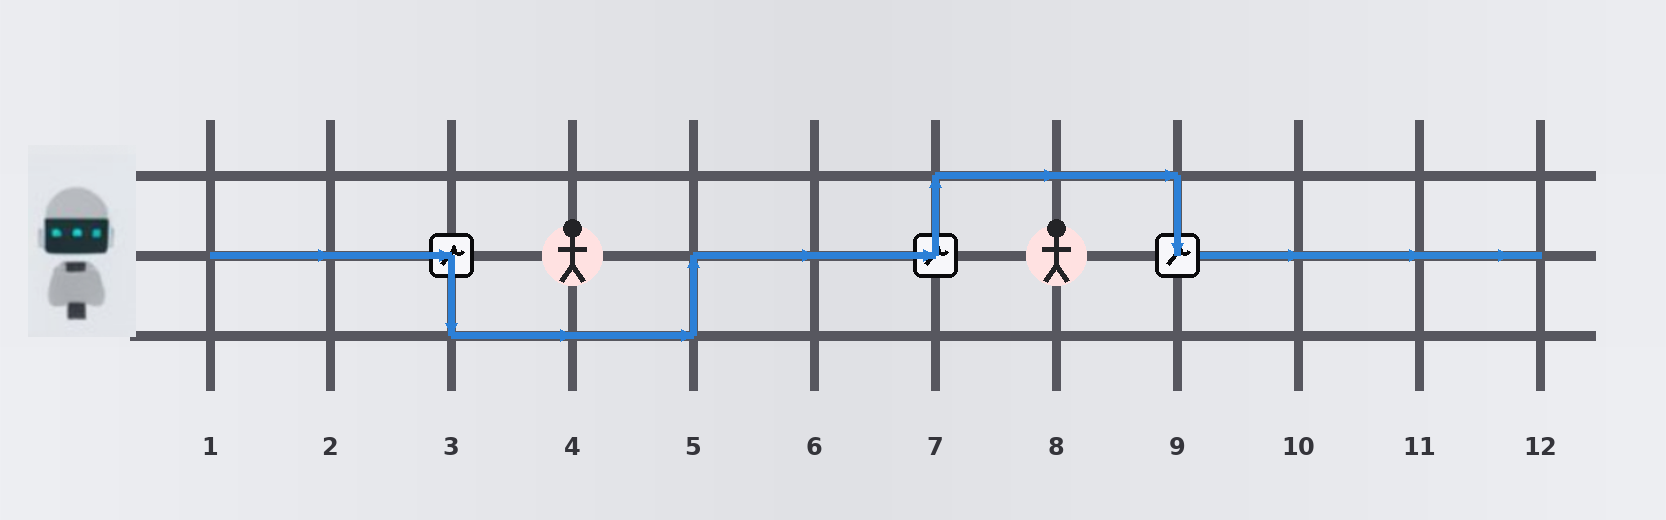
\includegraphics[width=\textwidth]{figures/robot6.png}
\caption{Example \ref{ex3}: A three-lane production corridor with required service cells at columns 3, 7, and 9 (middle lane), occupied crossing cells at columns 4 and 8, and terminal target at column 12 in the middle lane. The highlighted route shows a collision-free detour using lane changes and continuation to the terminal cell.}\label{f-ex3}
\Description{A three-lane corridor with 12 columns. The robot starts at column 1 in the middle lane, services columns 3, 7, and 9, detours around occupied middle-lane cells at columns 4 and 8, and finally reaches column 12 in the middle lane.}
\end{center}
\end{figure}

The previous examples are effectively one-dimensional: intersections are ordered along a road.
We now show a two-dimensional setting that still satisfies the locality assumptions when one dimension is small.
Consider a long production line with $n$ columns and $W$ parallel conveyor lanes, where $W$ is a fixed small constant (eg, $W=3$). The robot can move forward along the line and switch between neighboring lanes, while human workers may temporarily occupy specific crossing cells that must be avoided.

Figure \ref{f-ex3} illustrates the concrete instance used in this subsection. The robot starts in the middle lane at column 1. Required service cells are in the middle lane at columns 3, 7, and 9, while human-occupied cells appear in the middle lane at columns 4 and 8. A direct middle-lane traversal would enter those occupied cells and violate safety. Therefore, after repairing column 3, the robot detours to another lane before column 4 and returns to the middle lane afterward; later it performs an analogous detour around column 8 before returning to repair column 9. After completing the required repairs, it must continue to the terminal target cell at column 12 in the middle lane.

We index each cell by $(i,y)$ where $i\in\{1,\dots,n\}$ is the column and $y\in\{1,\dots,W\}$ is the lane.
The key modeling choice is to map locality to columns, ie, we define $loc(\cdot)=i$ for every proposition indexed by $(i,y)$.
This keeps the "long" direction explicit, while the lane index is absorbed into the bounded number of propositions per location.
Formally,
\begin{equation}
\begin{aligned}
Loc = \bigcup_{i=1}^n \{robot_{i,y}, done_{i,y}, human_{i,y}: y=1,\dots,W\},\\
Glob=\{collision\}.
\end{aligned}
\end{equation}
Hence each location $i$ has at most $3W$ local propositions, so $M=3W$ is constant when $W$ is fixed.

Let $R\subseteq \{1,\dots,n\}\times\{1,\dots,W\}$ be the set of stations that must be serviced.
The value set is
\begin{equation}
\Omega=\{G\neg collision\}\ \cup\ \{FG\,done_{i,y}:(i,y)\in R\}\ \cup\ \{FG\,robot_{n,2}\}.
\end{equation}
Thus, collisions are always forbidden, every required station must eventually be repaired and remain repaired, and the robot must eventually reach and remain at the terminal middle-lane cell $(n,2)$.

We use three action families:
\begin{itemize}
    \item {\it Forward move} $m_{i,y}$ for $1\le i<n$: move from $(i,y)$ to $(i+1,y)$.
    \item {\it Lane change} $s_{i,y\to y'}$ for $|y-y'|=1$: move at fixed column $i$ from lane $y$ to lane $y'$.
    \item {\it Repair} $rep_{i,y}$: repair station at $(i,y)$.
\end{itemize}
Representative effects are:
\begin{equation}
\begin{aligned}
\gamma^-(m_{i,y},robot_{i,y})&=robot_{i,y},\\
\gamma^+(m_{i,y},robot_{i+1,y})&=robot_{i,y},\\
\gamma^+(m_{i,y},collision)&=robot_{i,y}\land human_{i+1,y}.
\end{aligned}
\end{equation}
\begin{equation}
\begin{aligned}
\gamma^-(s_{i,y\to y'},robot_{i,y})&=robot_{i,y},\\
\gamma^+(s_{i,y\to y'},robot_{i,y'})&=robot_{i,y},\\
\gamma^+(s_{i,y\to y'},collision)&=robot_{i,y}\land human_{i,y'}.
\end{aligned}
\end{equation}
\begin{equation}
\begin{aligned}
\gamma^+(rep_{i,y},done_{i,y})&=robot_{i,y}\land \neg human_{i,y},\\
\gamma^+(rep_{i,y},collision)&=robot_{i,y}\land human_{i,y}.
\end{aligned}
\end{equation}
For the concrete three-lane encoding ($A,B,C$), these schemas ground to the input rules. In particular, collision updates include
\begin{equation}
\begin{aligned}
\gamma^+(mA_i,collision)&=ra_i\land ha_{i+1},\quad
\gamma^+(mB_i,collision)=rb_i\land hb_{i+1},\quad
\gamma^+(mC_i,collision)=rc_i\land hc_{i+1},\\
\gamma^+(sAB_i,collision)&=ra_i\land hb_i,\quad
\gamma^+(sBA_i,collision)=rb_i\land ha_i,\quad
\gamma^+(sBC_i,collision)=rb_i\land hc_i,\\
\gamma^+(sCB_i,collision)&=rc_i\land hb_i.
\end{aligned}
\end{equation}
Likewise, movement effects are source-conditioned (e.g., $\gamma^-(mA_i,ra_i)=ra_i$ and $\gamma^+(mA_i,ra_{i+1})=ra_i$), which exactly matches rules such as ``\texttt{+ mA1 collision : ra1 AND ha2}'' in the instantiated specification.
All other effects are $\bot$. In this model, move actions touch only columns $i$ and $i+1$, lane changes and repairs touch only column $i$, and all of them may touch one global proposition ($collision$). Therefore $r(a)-l(a)\le 1$ for all actions, so the locality requirement is satisfied for $L=2$.

For the concrete instance from Figure \ref{f-ex3}, let $n=12$, $W=3$, $R=\{(3,2),(7,2),(9,2)\}$, and let the initial robot position be $(1,2)$.
Crossing zones $(4,2)$ and $(8,2)$ are occupied by humans.
A satisfying plan is:
\begin{equation*}
\begin{split}
\pi = (&m_{1,2}, m_{2,2}, rep_{3,2}, s_{3,2\to 3}, m_{3,3}, m_{4,3}, s_{5,3\to 2},\\
      &m_{5,2}, m_{6,2}, rep_{7,2}, s_{7,2\to 1}, m_{7,1}, m_{8,1}, s_{9,1\to 2}, rep_{9,2},\\
      &m_{9,2}, m_{10,2}, m_{11,2}).
\end{split}
\end{equation*}
The robot repairs required cells, detours around occupied crossing zones by switching lanes before entering unsafe cells, and then continues to the terminal target $B12$.
This example is two-dimensional in geometry, but remains one-dimensional in locality indexing with a fixed-width augmentation, which is exactly the regime targeted by our complexity assumptions.

\section{Evaluation}\label{eval}

This section evaluates whether the theoretical locality advantage translates into practical runtime gains. We compare three planners under a common protocol: the proposed locality-based planner, a brute-force planner with online value pruning, and an automata/progression $LTL_f$ baseline. The automata/progression baseline follows the standard finite-trace temporal-logic approach in which search is performed on a product between planning states and temporal-monitor states \cite{degiacomo2013ltlf,camacho2018finite}; operationally, each value formula is represented by a residual formula that is progressed after each action. In all experiments, every produced plan is checked by an independent validator, so correctness is not inferred from internal planner state.

\subsection{Setup}

All experiments were run on an Intel Core i7-10510U (4 cores / 8 threads) machine with 31\,GiB RAM, Ubuntu Linux kernel 5.15, and C++17 implementations compiled with \texttt{g++ 9.4.0} using optimization level \texttt{-O2}.
Code, benchmark-generation scripts, and experiment artifacts are available at \url{https://github.com/satja/LTL}.

The benchmark set consists of 110 systematically generated instances with problem size $n\in[6,16]$ and ten instances per size. The generation procedure is deterministic and size-ordered, with nontrivial pattern variation per size: damaged-location patterns in Example 1 and Example 2, and service/occupied-cell patterns in Example 3. Each family is generated from the same action/value definitions used in its corresponding example subsection, including the one-charge policy in Example 2 and the source-conditioned lane/move effects in Example 3. Family assignment follows a fixed cyclic pattern over variants, yielding 44 instances from the linear traffic-light family (Example 1), 33 from the charging extension (Example 2), and 33 from the three-lane repair corridor (Example 3). This design provides controlled growth in instance size while preserving the locality assumptions studied in Section \ref{aa}, while also testing whether conclusions remain stable across all three modeling variants rather than only one. In the plots, this means that for each fixed $n$ there are exactly ten benchmark instances.

All methods are run with the same maximum search depth (160) and evaluated per instance under equal fixed runtime limits of 15 seconds per planner. The locality parameter is fixed at $L=3$, matching the largest locality width among the benchmark families. Example \ref{ex3} itself already satisfies locality for $L=2$, but we keep a single fixed $L$ across all families for direct comparability. A run is counted as successful only if a planner returns a plan within the time limit and that plan is accepted by independent validation. Reported planning times exclude validation time, so runtime values represent planner-only cost.

\subsection{Results}

Table \ref{t:eval} summarizes success counts and runtime statistics on the full 110-instance suite. The locality-based planner solves all 110 instances within the 15-second limit, and all 110 successful outputs are validated. The automata/progression baseline solves 105 instances and times out on 5, with all 105 successful outputs validated. The brute-force baseline solves 90 instances and times out on 20, with all 90 successful outputs validated. Runtime statistics are computed over successful runs only: the locality planner has mean runtime 0.018s, median 0.00s, and maximum 0.12s; the automata/progression baseline has mean 0.572s, median 0.03s, and maximum 12.05s; and the brute-force baseline has mean 1.576s, median 0.25s, and maximum 13.81s.

To test whether the runtime advantage is statistically significant at the distribution level, we apply one-sided Mann--Whitney U tests with alternative hypothesis that locality runtimes are smaller than baseline runtimes. Using per-instance planner times (including timeout-capped values), we obtain $p=1.86\times 10^{-31}$ for locality versus brute force and $p=3.90\times 10^{-14}$ for locality versus automata/progression. Under this equal-timeout setting, locality is significantly faster than both baselines in the capped per-instance distribution.
Because all three methods use the same 15-second timeout cap, the rank-based comparison does not depend on asymmetric censoring thresholds.

\begin{table}[ht!]
\centering
\caption{Benchmark summary over 110 instances (successful runs only for runtime statistics).}
\label{t:eval}
\begin{tabular}{lccccc}
\toprule
Method & Success & Timeout & Mean (s) & Median (s) & Max (s) \\
\midrule
Locality-based planner & 110/110 & 0 & 0.018 & 0.00 & 0.12 \\
Automata/progression baseline & 105/110 & 5 & 0.572 & 0.03 & 12.05 \\
Brute-force baseline & 90/110 & 20 & 1.576 & 0.25 & 13.81 \\
\bottomrule
\end{tabular}
\end{table}

To make the cross-example effect explicit, Table \ref{t:eval-families} reports success counts separately for the three benchmark families. The locality planner remains complete in each family under the common 15-second cap. The automata/progression baseline is complete on Example 1 and Example 3, and loses robustness on Example 2. Brute force times out on a subset of Example 1 and on roughly half of Example 2, while remaining complete on Example 3 in this suite.

\begin{table}[ht!]
\centering
\caption{Success counts by benchmark family (timeout limit: 15s for all methods).}
\label{t:eval-families}
\begin{tabular}{lccc}
\toprule
Family & Locality-based & Automata/progression & Brute-force \\
\midrule
Example 1 (linear traffic lights, 44 instances) & 44/44 & 44/44 & 41/44 \\
Example 2 (charging extension, 33 instances) & 33/33 & 28/33 & 16/33 \\
Example 3 (three-lane corridor, 33 instances) & 33/33 & 33/33 & 33/33 \\
\bottomrule
\end{tabular}
\end{table}

\begin{figure}[ht!]
\begin{center}
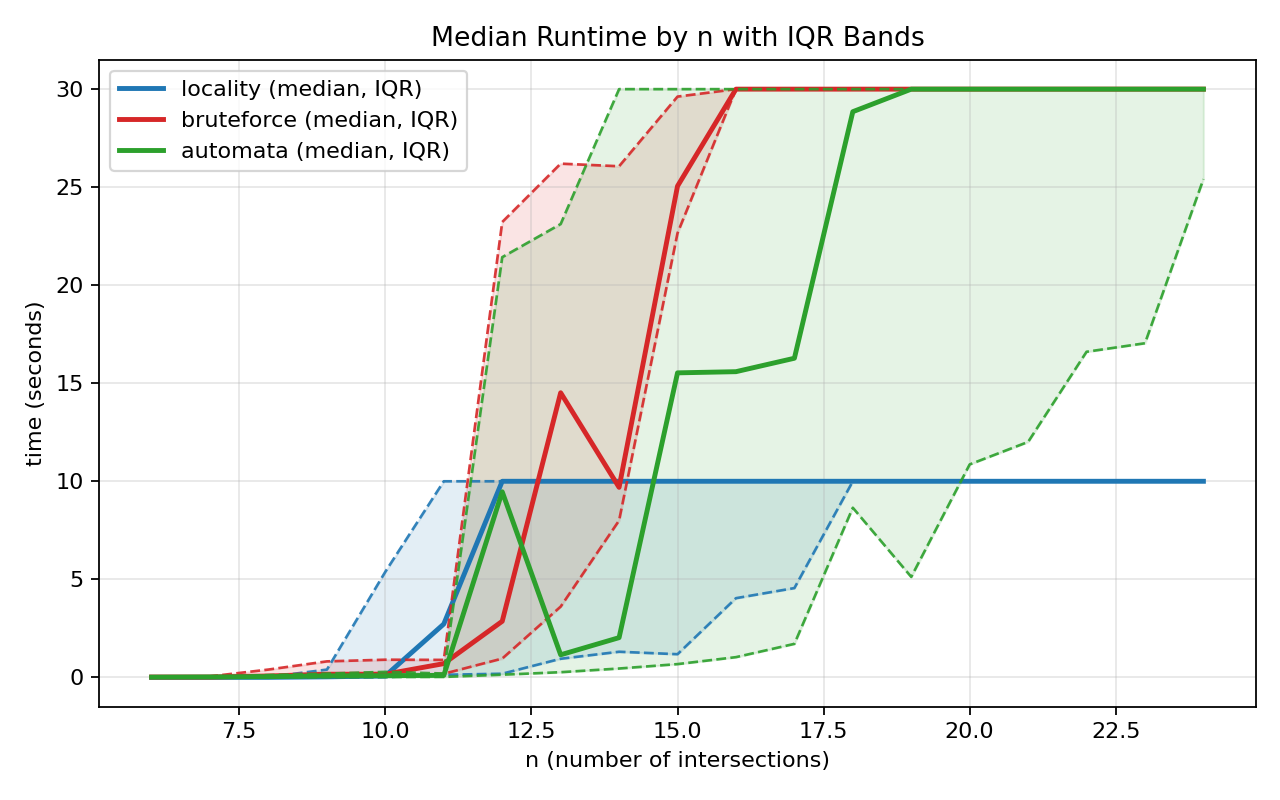
\includegraphics[width=0.82\textwidth]{figures/benchmark-time-median-iqr-vs-n.png}
\caption{Runtime versus instance size $n$ with ten instances per size. Solid lines show median runtime for each method and dashed side lines show the first and third quartiles (IQR band).}
\label{f3}
\Description{Runtime by instance size for locality, brute-force, and automata/progression planners. Each method is shown with a median line and dashed first/third quartile lines.}
\end{center}
\end{figure}

\begin{figure}[ht!]
\begin{center}
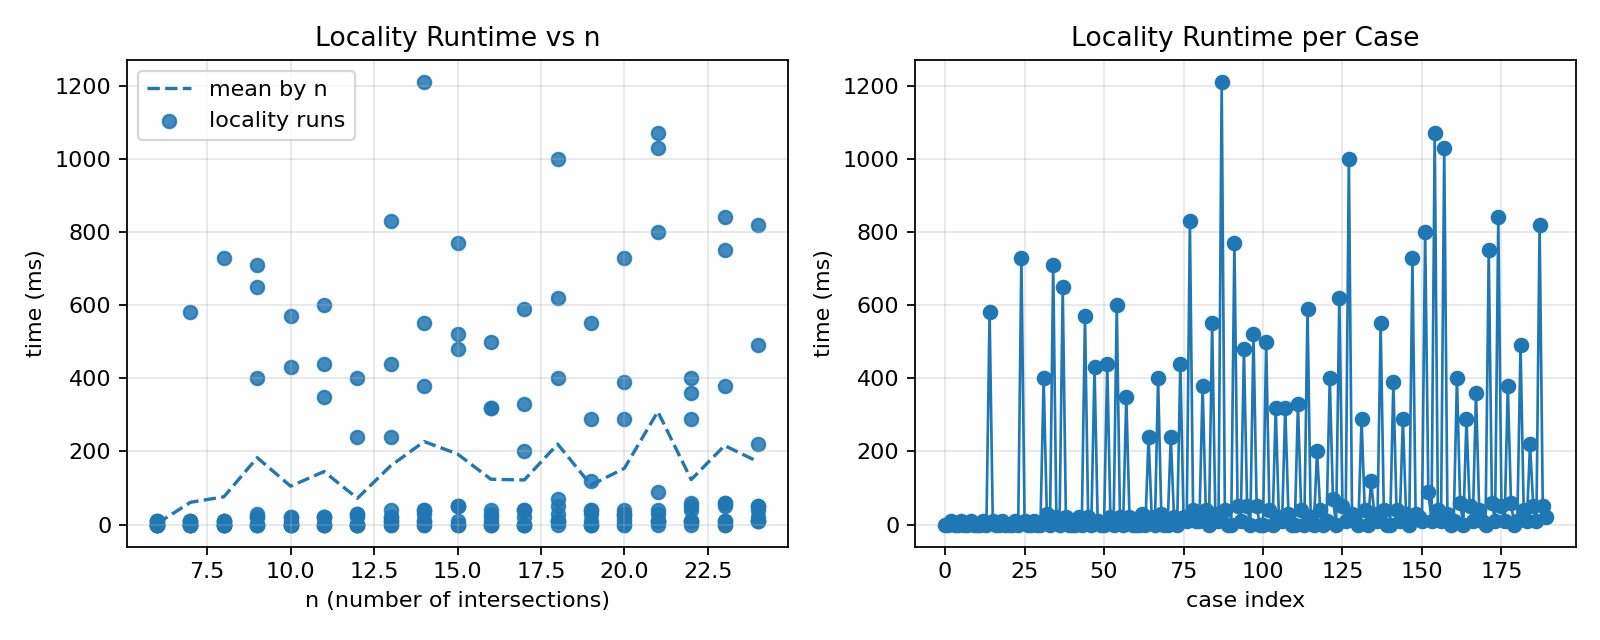
\includegraphics[width=0.82\textwidth]{figures/benchmark-time-locality.png}
\caption{Locality-only runtime detail. The left panel shows all locality runs grouped by $n$ with the mean trend, and the right panel shows the same runs by case index. Isolating this method reveals its internal growth pattern that is visually compressed in the multi-method comparison.}
\label{f3local}
\Description{Two-panel runtime plot for the locality planner only: scatter and trend by size in the left panel, and per-case runtime in the right panel.}
\end{center}
\end{figure}

\subsection{Results Discussion}

The central empirical observation is that locality-aware state compression dominates in this benchmark regime. Under the fixed setting $L=3$ and a common 15-second budget, the locality planner solves all instances and has the lowest runtime distribution. This matters because the three families stress different parts of the model: the first emphasizes local repair propagation with global congestion safety, the second adds charging-related propositions and additional temporal obligations, and the third introduces lane switches and collision-avoidance structure in a narrow two-dimensional geometry.
Figure \ref{f3} provides the aggregate view by number of intersections using robust summary statistics: for each method, the median runtime grows with $n$, and the dashed bands show the interquartile range. Figure \ref{f3local} complements this by isolating only the locality planner. This view confirms that locality runtime remains low across the full size range, including larger instances in the suite.

The baseline behavior is heterogeneous by family, which helps explain aggregate statistics. On Example 1, locality and automata/progression are both complete, while brute force loses robustness on a small subset. On Example 2, locality is complete, automata/progression times out on a nontrivial subset, and brute force times out on roughly half of instances. On Example 3, all three methods are complete under the 15-second budget, but locality still maintains the lowest runtime distribution.

These results are consistent with the theory from Section \ref{pa}. The proposed method keeps only a bounded active window of local propositions, together with global propositions and compact temporal-status memory, and shifts this window left-to-right. In this locality-structured benchmark, that representation yields both strong pruning and low per-state overhead, which explains the observed runtime and completion advantage. The automata/progression baseline, by construction, explores product states that combine planning valuations with residual temporal formulas, and this temporal-monitor overhead is most visible in the charger family where temporal obligations are denser. The brute-force baseline suffers most from direct state-space growth, despite online pruning.

At the same time, interpretation should remain scoped to the evaluated regime. All three families are locality-structured by design and therefore aligned with the assumptions of our algorithm. This is appropriate for validating the intended use case and stronger than evaluating only one family, but it is still not evidence that the same margins will hold on domains with weak locality or substantially different temporal-value distributions. %A broader study with additional non-local families, parameter sweeps over $L$, and cross-platform timing would provide a stronger estimate of external validity.

\section{Conclusion}\label{conc}

We introduced a locality-based approach to solving the CONFLICT problem in ethical planning using Linear Temporal Logic (LTL). By incorporating assumptions on the structure of the problem, the distinction between global and local propositions and the constraints on the scope and sequence of actions, we were able to reduce the complexity of the problem from PSPACE-complete to polynomial time. The introduced concept of localized planning restricts the actions to only affect and depend on propositions within a bounded interval. It incorporates constraints on the temporal order of actions based on this interval. Due to possibility of large constant factors in the algorithm complexity, there might be a tradeoff between efficiency and flexibility. We consider the proposed algorithm to be practical   for real-world applications with small values of constants $K$, $L$, and $M$, ie, the applications with "high locality".
The evaluation in Section \ref{eval} supports this claim by showing both runtime and robustness advantages on the systematic locality-structured benchmark suite.

Overall, our work offers a promising direction for efficient and scalable ethical planning in autonomous systems and robotics. By constraining the problem space in a principled way, we enable the development of action plans that adhere to predefined values, ensuring ethical behavior in complex, dynamic environments. Future research could explore extending this framework to accommodate more complex moral structures and larger sets of global propositions, as well as applying these methods to real-world robotic systems and other automated decision-making contexts.


%\begin{acks}
%To Robert, for the bagels and explaining CMYK and color spaces.
%\end{acks}

%%
%% The next line prints the references.
\printbibliography


%%
%% If your work has an appendix, this is the place to put it.
%\appendix


%\section{Research Methods}

%\subsection{Part One}

%Lorem ipsum dolor sit amet, consectetur adipiscing elit. Morbi
%malesuada, quam in pulvinar varius, metus nunc fermentum urna, id
%sollicitudin purus odio sit amet enim. Aliquam ullamcorper eu ipsum
%vel mollis. Curabitur quis dictum nisl. Phasellus vel semper risus, et
%lacinia dolor. Integer ultricies commodo sem nec semper.

%\subsection{Part Two}

%Etiam commodo feugiat nisl pulvinar pellentesque. Etiam auctor sodales
%ligula, non varius nibh pulvinar semper. Suspendisse nec lectus non
%ipsum convallis congue hendrerit vitae sapien. Donec at laoreet
%eros. Vivamus non purus placerat, scelerisque diam eu, cursus
%ante. Etiam aliquam tortor auctor efficitur mattis.

%\section{Online Resources}

%Nam id fermentum dui. Suspendisse sagittis tortor a nulla mollis, in
%pulvinar ex pretium. Sed interdum orci quis metus euismod, et sagittis
%enim maximus. Vestibulum gravida massa ut felis suscipit
%congue. Quisque mattis elit a risus ultrices commodo venenatis eget
%dui. Etiam sagittis eleifend elementum.

%Nam interdum magna at lectus dignissim, ac dignissim lorem
%rhoncus. Maecenas eu arcu ac neque placerat aliquam. Nunc pulvinar
%massa et mattis lacinia.

\appendix
\section{Reproducibility Checklist for JAIR}

Select the answers that apply to this research.

\subsection*{All articles}
\begin{enumerate}
    \item All claims investigated in this work are clearly stated. [yes]
    \item Clear explanations are given how the work reported substantiates the claims. [yes]
    \item Limitations or technical assumptions are stated clearly and explicitly. [yes]
    \item Conceptual outlines and/or pseudo-code descriptions of the AI methods introduced in this work are provided, and important implementation details are discussed. [yes]
    \item Motivation is provided for all design choices, including algorithms, implementation choices, parameters, data sets and experimental protocols beyond metrics. [yes]
\end{enumerate}

\subsection*{Articles containing theoretical contributions}
Does this paper make theoretical contributions? [yes]
\begin{enumerate}
    \item All assumptions and restrictions are stated clearly and formally. [yes]
    \item All novel claims are stated formally (e.g., in theorem statements). [yes]
    \item Proofs of all non-trivial claims are provided in sufficient detail to permit verification by readers with a reasonable degree of expertise. [partially]
    \item Complex formalism, such as definitions or proofs, is motivated and explained clearly. [yes]
    \item The use of mathematical notation and formalism serves the purpose of enhancing clarity and precision; gratuitous use of mathematical formalism is avoided. [yes]
    \item Appropriate citations are given for all non-trivial theoretical tools and techniques. [yes]
\end{enumerate}

\subsection*{Articles reporting on computational experiments}
Does this paper include computational experiments? [yes]
\begin{enumerate}
    \item All source code required for conducting experiments is included in an online appendix or will be made publicly available upon publication of the paper. [yes]
    \item The source code comes with a license that allows free usage for reproducibility purposes. [yes]
    \item The source code comes with a license that allows free usage for research purposes in general. [yes]
    \item Raw, unaggregated data from all experiments is included in an online appendix or will be made publicly available upon publication of the paper. [yes]
    \item The unaggregated data comes with a license that allows free usage for reproducibility purposes. [yes]
    \item The unaggregated data comes with a license that allows free usage for research purposes in general. [yes]
    \item If an algorithm depends on randomness, then the method used for generating random numbers and for setting seeds is described in a way sufficient to allow replication of results. [yes]
    \item The execution environment for experiments, including hardware and software stack, is described. [yes]
    \item The evaluation metrics used in experiments are clearly explained and their choice is explicitly motivated. [yes]
    \item The number of algorithm runs used to compute each result is reported. [yes]
    \item Reported results have not been ``cherry-picked'' by silently ignoring unsuccessful or unsatisfactory experiments. [yes]
    \item Analysis of results goes beyond single-dimensional summaries of performance to include measures of variation, confidence, or other distributional information. [yes]
    \item All (hyper-) parameter settings for the algorithms/methods used in experiments have been reported, along with the rationale or method for determining them. [yes]
    \item The number and range of (hyper-) parameter settings explored prior to conducting final experiments have been indicated, along with the effort spent on (hyper-) parameter optimisation. [partially]
    \item Appropriately chosen statistical hypothesis tests are used to establish statistical significance in the presence of noise effects. [yes]
\end{enumerate}

\subsection*{Articles using data sets}
Does this work rely on one or more data sets (possibly obtained from a benchmark generator or similar software artifact)? [yes]
\begin{enumerate}
    \item All newly introduced data sets are included in an online appendix or will be made publicly available upon publication of the paper. [yes]
    \item The newly introduced data set comes with a license that allows free usage for reproducibility purposes. [yes]
    \item The newly introduced data set comes with a license that allows free usage for research purposes in general. [yes]
    \item All data sets drawn from the literature or other public sources are accompanied by appropriate citations. [NA]
    \item All data sets drawn from the existing literature are publicly available. [NA]
    \item All new data sets and data sets that are not publicly available are described in detail, including relevant statistics and data collection process if relevant. [yes]
    \item All methods used for preprocessing, augmenting, batching or splitting data sets are described in detail. [NA]
\end{enumerate}

\subsection*{Explanations on answers above (optional)}
Code and benchmark artifacts are available in the project repository and released under the MIT License.

\end{document}
\endinput
%%
%% End of file `sample-acmlarge.tex'.
